\hypertarget{curious-george-doll}{%
\section{Curious George doll}\label{curious-george-doll}}

\begin{figure}[!ht]
  \begin{adjustwidth}{-\oddsidemargin-1in}{-\rightmargin}
    \centering
    
\includegraphics[trim={0 6cm 0 2cm,}, clip, width=\paperwidth]{./S01/img/21/curious-george-doll.png}
    % \caption{Curious George doll\label{fig:curious-george-doll}}
  \end{adjustwidth}
\end{figure}

\begin{tcolorbox}[enhanced,center upper,
    drop fuzzy shadow southeast, boxrule=0.3pt,
    lower separated=false, breakable,
    colframe=black!30!dialogoBorder,colback=white]
\begin{minipage}[c]{0.16\linewidth}
  \raisebox{\dimexpr-\height+\ht\strutbox\relax}{
    \centering 
\includegraphics[width=1.4cm]{./assets/img/rachel.png}
  }
   & \centering \scriptsize{Rachel}
\end{minipage}
\hfill
\begin{minipage}[c]{0.8\linewidth}
  \textbf{- Marcel, stop it! Marcel! Bad monkey!}\\
  - Marcel, para! Marcel! Macaco malvado!
\end{minipage}

\medskip
\begin{minipage}[c]{0.16\linewidth}
  \raisebox{\dimexpr-\height+\ht\strutbox\relax}{
    \centering 
\includegraphics[width=1.4cm]{./assets/img/ross.png}
  }
   & \centering \scriptsize{Ross}
\end{minipage}
\hfill
\begin{minipage}[c]{0.8\linewidth}
  \textbf{- What?}\\
  - Que foi?
\end{minipage}

\medskip
\begin{minipage}[c]{0.16\linewidth}
  \raisebox{\dimexpr-\height+\ht\strutbox\relax}{
    \centering 
\includegraphics[width=1.4cm]{./assets/img/rachel.png}
  }
   & \centering \scriptsize{Rachel}
\end{minipage}
\hfill
\begin{minipage}[c]{0.8\linewidth}
  \textbf{- Let's just say my Curious George doll is no longer curious.}\\
  - Meu boneco George Curioso não está mais curioso.
\end{minipage}
\end{tcolorbox}

Em sua fase de cio Marcel ``se diverte'' com um boneco da Rachel,
\emph{Curious George} (1941), personagem criado pelo casal \emph{Hans
Augusto Rey} (1898-1977) e \emph{Margret Rey} (1906-1996) em livro
homônimo. O macaquinho ainda estrolou uma série de 6 livros, um
longa-metragem, vídeo \emph{games} e uma série de TV, além, é claro, dos
bonecos de pelúcia.

\begin{figure}
  \centering
  \begin{tikzpicture}
    \node [inner sep=0pt] at (0,0) {
      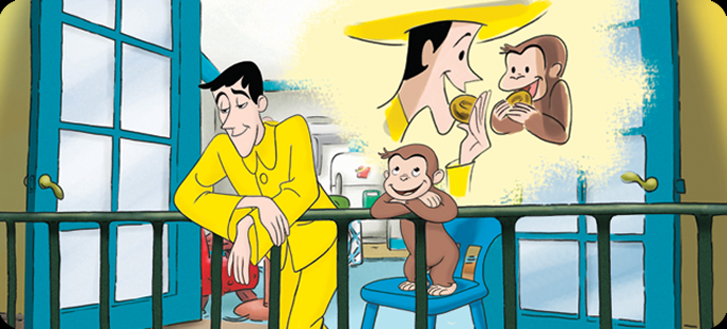
\includegraphics[width=0.8\textwidth,keepaspectratio]{./S01/img/21/curious-george-tv.png}
    };
    \draw [white, rounded corners=\ClipSep, line width=\ClipSep]
    (current bounding box.north west) --
    (current bounding box.north east) --
    (current bounding box.south east) --
    (current bounding box.south west) -- cycle
    ;
    \end{tikzpicture}
    \caption{Curious George TV\label{fig:curious-george-tv}}
\end{figure}

\hypertarget{referuxeancias}{%
\subsection{Referências}\label{referuxeancias}}

\begin{itemize}
\tightlist
\item
  \sloppy Curious George - Site oficial (Inglês). \url{https://www.curiousgeorge.com/about%20us}
\end{itemize}

\hypertarget{fiddler-on-the-roof}{%
\section{Fiddler on the Roof}\label{fiddler-on-the-roof}}

\begin{figure}[!ht]
  \begin{adjustwidth}{-\oddsidemargin-1in}{-\rightmargin}
    \centering
    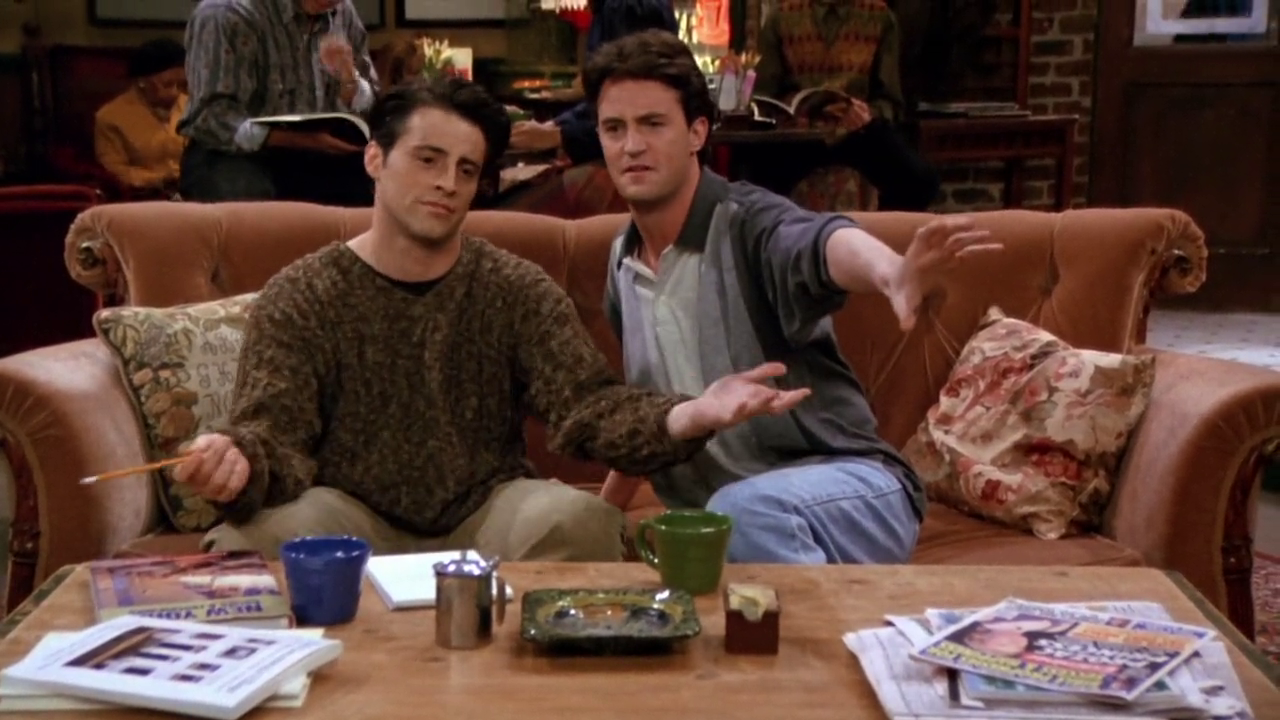
\includegraphics[trim={0 7cm 0 1cm,}, clip, width=\paperwidth]{./S01/img/21/fiddler-on-the-roof.png}
    % \caption{Fiddler on the Roof\label{fig:fiddler-on-the-roof}}
  \end{adjustwidth}
\end{figure}

\begin{tcolorbox}[enhanced,center upper,
    drop fuzzy shadow southeast, boxrule=0.3pt,
    lower separated=false, breakable,
    colframe=black!30!dialogoBorder,colback=white]
\begin{minipage}[c]{0.16\linewidth}
  \raisebox{\dimexpr-\height+\ht\strutbox\relax}{
    \centering 
\includegraphics[width=1.4cm]{./assets/img/chandler.png}
  }
   & \centering \scriptsize{Chandler}
\end{minipage}
\hfill
\begin{minipage}[c]{0.8\linewidth}
  \textbf{- Joseph Stalin is the Fiddler on the Roof.}\\
  - Joseph Stalin é Um Violinista no Telhado.
\end{minipage}
\end{tcolorbox}

Joey busca um nome artístico, a pedido de sua agente. Chandler sugere
\emph{Joseph Stalin} (1878-1953), e demonstra como seria a chamada do
musical \emph{Fiddler on the Roof} (1964), uma produção original da
\emph{Broadway}, o famoso teatro localizado no centro de
\emph{Manhattan}. O musical, mais tarde, foi adaptado para um filme de
mesmo nome (1971) e conta a história de um camponês judeu que vive na
Rússia pré-revolucionária, e luta contra o casamento de três de suas
filhas, ao mesmo tempo que um sentimento anti-semita ameaça a vila onde
mora.

Na mesma cena Chandler menciona \emph{Bye Bye Birdie}, que já foi citado
no episódio
\textbf{\textcolor{primarycolor}{S01E18 - Aquele com o Pôquer}}.

\emph{Joseph Stalin} é explicado mais tarde no próprio episódio por
Joey.

\begin{tcolorbox}[enhanced,center upper,
    drop fuzzy shadow southeast, boxrule=0.3pt,
    lower separated=false, breakable,
    colframe=black!30!dialogoBorder,colback=white]
\begin{minipage}[c]{0.16\linewidth}
  \raisebox{\dimexpr-\height+\ht\strutbox\relax}{
    \centering 
\includegraphics[width=1.4cm]{./assets/img/joey.png}
  }
   & \centering \scriptsize{Joey}
\end{minipage}
\hfill
\begin{minipage}[c]{0.8\linewidth}
  \textbf{- You know there already is a Joseph Stalin?}\\
  - Sabiam que já existe um Joseph Stalin?
\end{minipage}

\medskip
\begin{minipage}[c]{0.16\linewidth}
  \raisebox{\dimexpr-\height+\ht\strutbox\relax}{
    \centering 
\includegraphics[width=1.4cm]{./assets/img/chandler.png}
  }
   & \centering \scriptsize{Chandler}
\end{minipage}
\hfill
\begin{minipage}[c]{0.8\linewidth}
  \textbf{- You're kidding!}\\
  - Tá brincando?
\end{minipage}

\medskip
\begin{minipage}[c]{0.16\linewidth}
  \raisebox{\dimexpr-\height+\ht\strutbox\relax}{
    \centering 
\includegraphics[width=1.4cm]{./assets/img/joey.png}
  }
   & \centering \scriptsize{Joey}
\end{minipage}
\hfill
\begin{minipage}[c]{0.8\linewidth}
  \textbf{- Apparently, he was this Russian dictator who slaughtered all these people!}\\
  - Aparentemente, era um ditador russo que matou um monte de gente.
\end{minipage}
\end{tcolorbox}

\hypertarget{referuxeancias-1}{%
\subsection{Referências}\label{referuxeancias-1}}

\begin{itemize}
\tightlist
\item
  \sloppy IMDB. \url{https://www.imdb.com/title/tt0067093/?ref_=nv_sr_srsg_0}
\end{itemize}

\hypertarget{three-wise-monkeys}{%
\section{Three wise monkeys}\label{three-wise-monkeys}}

\begin{figure}[!ht]
  \begin{adjustwidth}{-\oddsidemargin-1in}{-\rightmargin}
    \centering
    
\includegraphics[trim={0 7cm 0 3cm,}, clip, width=\paperwidth]{./S01/img/21/three-wise-monkeys.png}
    % \caption{Three wise monkeys\label{fig:three-wise-monkeys}}
  \end{adjustwidth}
\end{figure}

Ross descobre que o cio de Marcel não é apenas uma fase e deverá doar o
macaco. Na cena há uma alusão ao provérbio japonês \emph{see no evil,
hear no evil, speak no evil}, que pode ser traduzido como \emph{não veja
o mal, não ouça o mal e não fale o mal}.

\hypertarget{referuxeancias-2}{%
\subsection{Referências}\label{referuxeancias-2}}

\begin{itemize}
\tightlist
\item
  \sloppy Wikipédia. \url{https://pt.wikipedia.org/wiki/Tr%C3%AAs_Macacos_S%C3%A1bios}
\end{itemize}

\hypertarget{dead-poets-society}{%
\section{Dead Poets Society}\label{dead-poets-society}}

\begin{figure}[!ht]
  \begin{adjustwidth}{-\oddsidemargin-1in}{-\rightmargin}
    \centering
    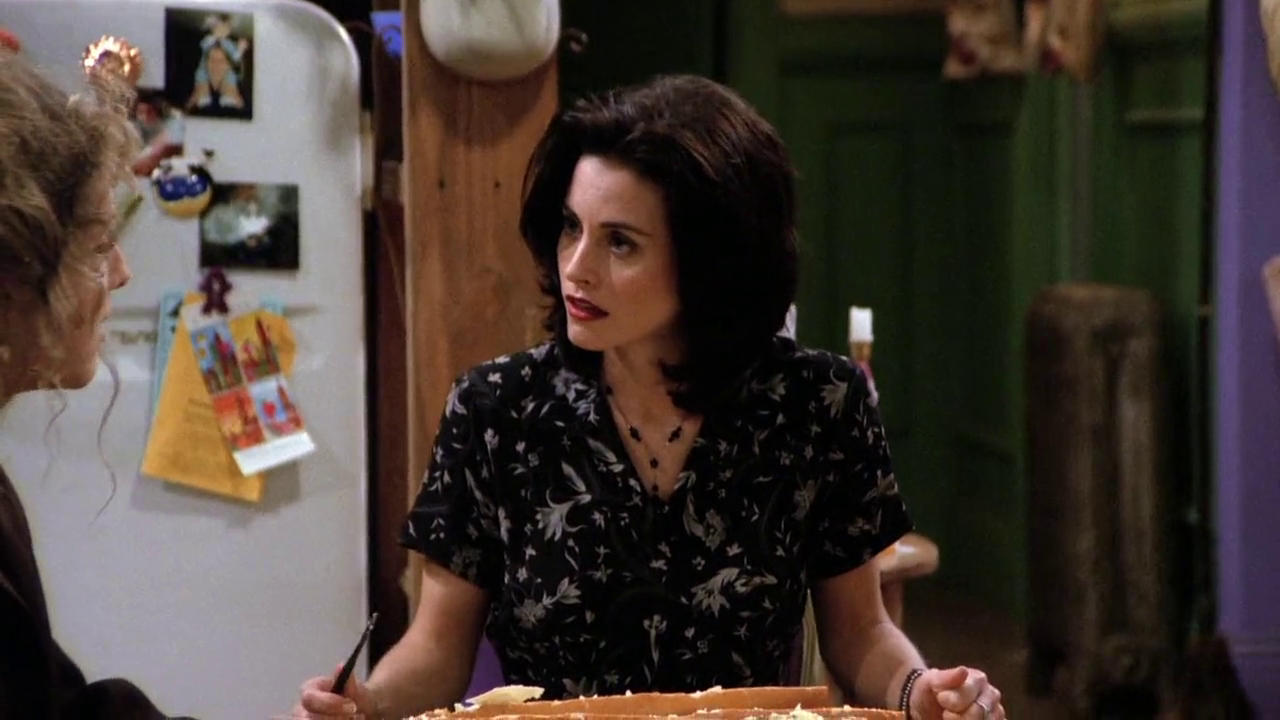
\includegraphics[trim={0 6cm 0 2cm,}, clip, width=\paperwidth]{./S01/img/21/dead-poets-society.png}
    % \caption{Dead Poets Society\label{fig:dead-poets-society}}
  \end{adjustwidth}
\end{figure}

\begin{tcolorbox}[enhanced,center upper,
    drop fuzzy shadow southeast, boxrule=0.3pt,
    lower separated=false, breakable,
    colframe=black!30!dialogoBorder,colback=white]
\begin{minipage}[c]{0.16\linewidth}
  \raisebox{\dimexpr-\height+\ht\strutbox\relax}{
    \centering 
\includegraphics[width=1.4cm]{./assets/img/fake-monica.png}
  }
   & \centering \scriptsize{M. Falsa}
\end{minipage}
\hfill
\begin{minipage}[c]{0.8\linewidth}
  \textbf{- Did you ever see Dead Poets Society?}\\
  - Viu A Sociedade dos Poetas Mortos?
\end{minipage}

\medskip
\begin{minipage}[c]{0.16\linewidth}
  \raisebox{\dimexpr-\height+\ht\strutbox\relax}{
    \centering 
\includegraphics[width=1.4cm]{./assets/img/monica.png}
  }
   & \centering \scriptsize{Monica}
\end{minipage}
\hfill
\begin{minipage}[c]{0.8\linewidth}
  \textbf{- Uh-huh.}\\
  - Não.
\end{minipage}

\medskip
\begin{minipage}[c]{0.16\linewidth}
  \raisebox{\dimexpr-\height+\ht\strutbox\relax}{
    \centering 
\includegraphics[width=1.4cm]{./assets/img/fake-monica.png}
  }
   & \centering \scriptsize{M. Falsa}
\end{minipage}
\hfill
\begin{minipage}[c]{0.8\linewidth}
  \textbf{- I thought that movie was so incredibly... boring!}\\
  - Achei aquele filme incrivelmente... chato!
\end{minipage}
\end{tcolorbox}

A Monica Falsa descreve como um filme mudou a vida dela, e menciona
\emph{Dead Poets Society} (1989), que conta a história de um ex-aluno de
uma escola ortodoxa que se torna professor de literatura e utiliza
métodos para fazer com que os alunos pensem por si próprios. No Brasil o
filme é conhecido como \emph{Sociedade dos Poetas Mortos}.

\begin{figure}
  \centering
  \begin{tikzpicture}
    \node [inner sep=0pt] at (0,0) {
      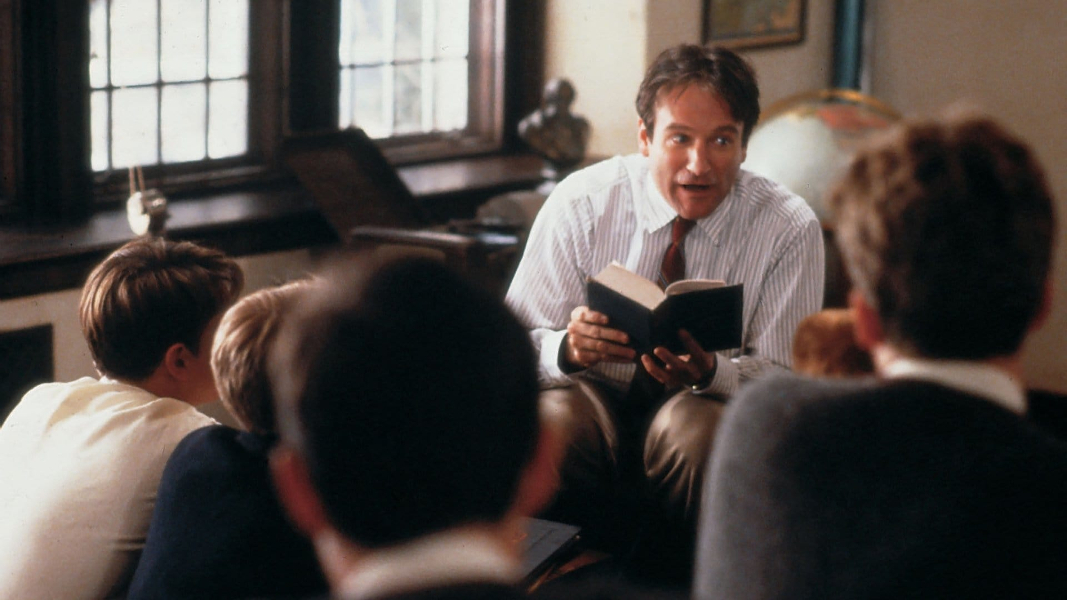
\includegraphics[width=0.8\textwidth,keepaspectratio]{./S01/img/21/dead-poets-society-filme.jpg}
    };
    \draw [white, rounded corners=\ClipSep, line width=\ClipSep]
    (current bounding box.north west) --
    (current bounding box.north east) --
    (current bounding box.south east) --
    (current bounding box.south west) -- cycle
    ;
    \end{tikzpicture}
    \caption{Dead Poets Society - Cena do filme\label{fig:dead-poets-society-cena-do-filme}}
\end{figure}

\hypertarget{referuxeancias-3}{%
\subsection{Referências}\label{referuxeancias-3}}

\begin{itemize}
\tightlist
\item
  \sloppy TMDB. \url{https://www.themoviedb.org/movie/207-dead-poets-society?language=pt-BR}
\end{itemize}

\hypertarget{mrs.-doubtfire}{%
\section{Mrs.~Doubtfire}\label{mrs.-doubtfire}}

\begin{figure}[!ht]
  \begin{adjustwidth}{-\oddsidemargin-1in}{-\rightmargin}
    \centering
    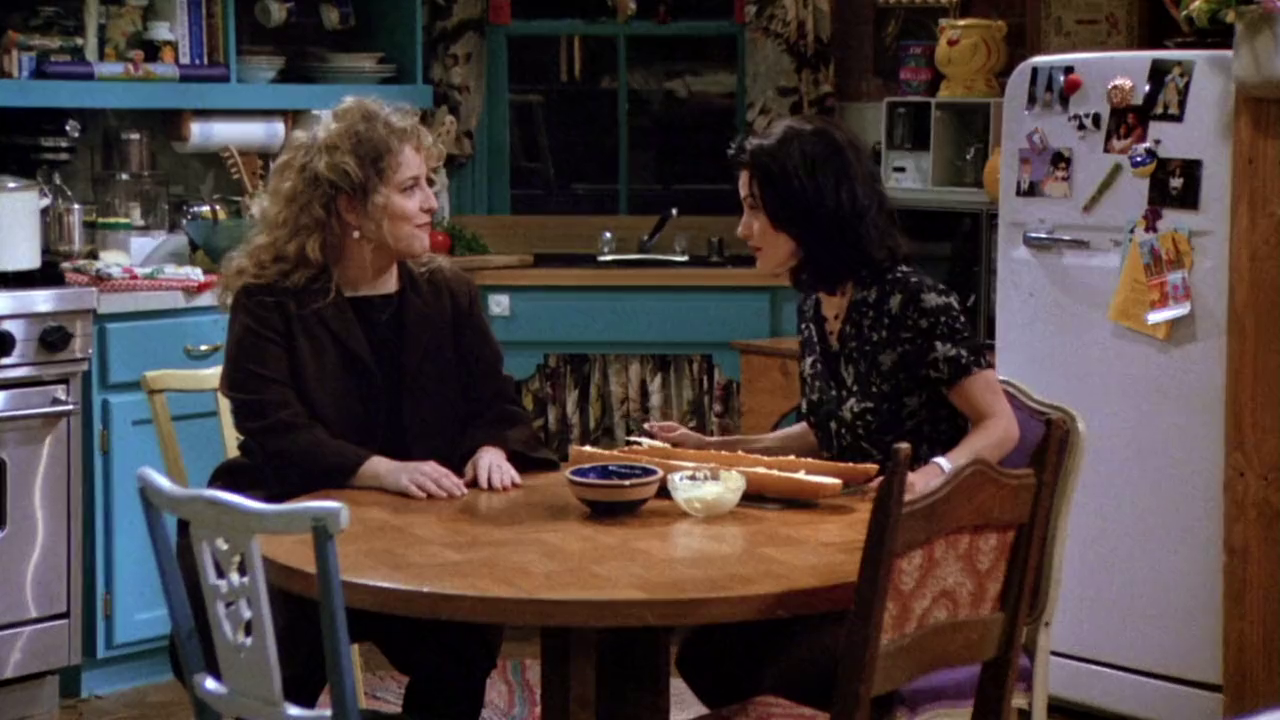
\includegraphics[trim={0 7cm 0 3cm,}, clip, width=\paperwidth]{./S01/img/21/mrs-doubtfire.png}
    % \caption{Mrs. Doubtfire\label{fig:mrs-doubtfire}}
  \end{adjustwidth}
\end{figure}

\begin{tcolorbox}[enhanced,center upper,
    drop fuzzy shadow southeast, boxrule=0.3pt,
    lower separated=false, breakable,
    colframe=black!30!dialogoBorder,colback=white]
\begin{minipage}[c]{0.16\linewidth}
  \raisebox{\dimexpr-\height+\ht\strutbox\relax}{
    \centering 
\includegraphics[width=1.4cm]{./assets/img/monica.png}
  }
   & \centering \scriptsize{Monica}
\end{minipage}
\hfill
\begin{minipage}[c]{0.8\linewidth}
  \textbf{- Then I would definitely not recommend Mrs. Doubtfire.}\\
  - Então, não veja Uma Babá Quase Perfeita.
\end{minipage}
\end{tcolorbox}

A Monica Falsa reclama como perdeu tempo de sua vida assistindo ao filme
\emph{Dead Poets Society} e a \emph{Monana} recomenda que ela não veja
\emph{Mrs.~Doubtfire} (1993), comédia que também é estrelada por
\emph{Robin Williams}. A trama envolve um sujeito que se separou e
arranja um emprego de babá em sua antiga casa disfarçado de uma senhora.

\begin{figure}
  \centering
  \begin{tikzpicture}
    \node [inner sep=0pt] at (0,0) {
      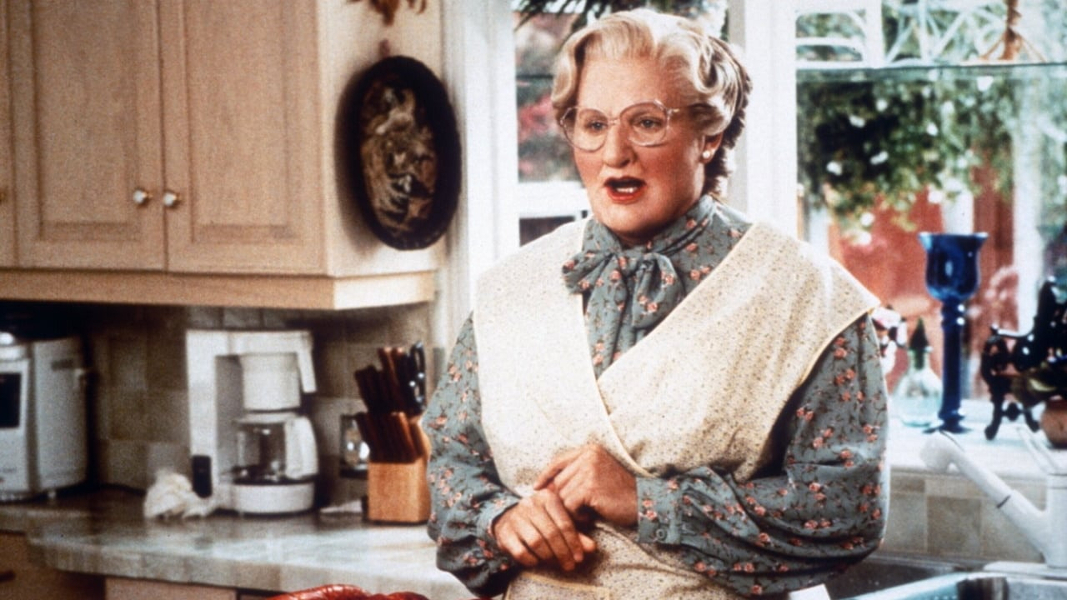
\includegraphics[width=0.8\textwidth,keepaspectratio]{./S01/img/21/mrs-doubtfire-filme.jpg}
    };
    \draw [white, rounded corners=\ClipSep, line width=\ClipSep]
    (current bounding box.north west) --
    (current bounding box.north east) --
    (current bounding box.south east) --
    (current bounding box.south west) -- cycle
    ;
    \end{tikzpicture}
    \caption{Mrs. Doubtfire - Cena do filme\label{fig:mrs-doubtfire-cena-do-filme}}
\end{figure}

\hypertarget{referuxeancias-4}{%
\subsection{Referências}\label{referuxeancias-4}}

\begin{itemize}
\tightlist
\item
  \sloppy TMDB. \url{https://www.themoviedb.org/movie/788-mrs-doubtfire}
\end{itemize}

\hypertarget{game-boy}{%
\section{Game Boy}\label{game-boy}}

\begin{figure}[!ht]
  \begin{adjustwidth}{-\oddsidemargin-1in}{-\rightmargin}
    \centering
    
\includegraphics[trim={0 5cm 0 4cm,}, clip, width=\paperwidth]{./S01/img/21/game-boy.png}
    % \caption{Game Boy\label{fig:game-boy}}
  \end{adjustwidth}
\end{figure}

Phoebe é vista em cena com um \emph{Game Boy} (1989), console portátil
da Nintendo, muito popular nos anos 90. Possui uma tela LCD com 4 tons
de cinza e sistema de cartuchos. Em seu lançamento nos EUA o console
vinha com o jogo \emph{Tetris}.

O fato dela estar com um \emph{Game Boy} pode ter relação com sua
resposta quando Joey pergunta que nome artístico seria legal, e ela
responde: \emph{``Flame Boy!''}.

\begin{figure}
  \centering
  \begin{tikzpicture}
    \node [inner sep=0pt] at (0,0) {
      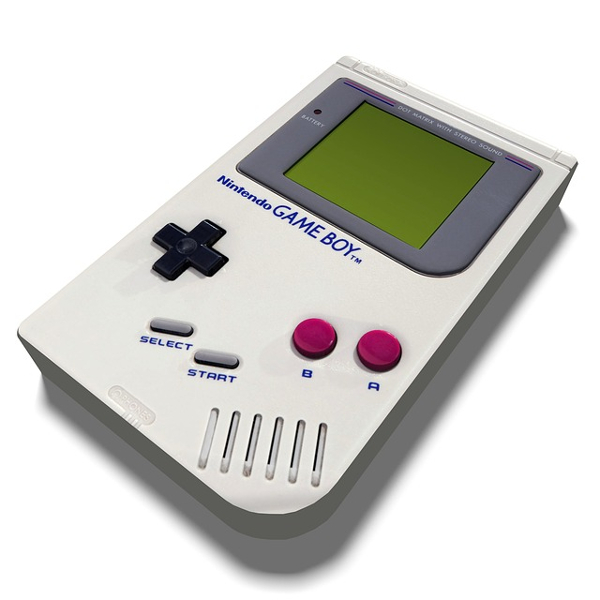
\includegraphics[width=0.5\textwidth,keepaspectratio]{./S01/img/21/gameboy-foto.jpg}
    };
    \draw [white, rounded corners=\ClipSep, line width=\ClipSep]
    (current bounding box.north west) --
    (current bounding box.north east) --
    (current bounding box.south east) --
    (current bounding box.south west) -- cycle
    ;
    \end{tikzpicture}
    \caption{Game Boy (Imagem de Alexander Antropov por Pixabay)\label{fig:game-boy-imagem-de-alexander-antropov-por-pixabay}}
\end{figure}

\hypertarget{referuxeancias-5}{%
\subsection{Referências}\label{referuxeancias-5}}

\begin{itemize}
\tightlist
\item
  \sloppy Site oficial da Nintendo (Inglês). \url{https://www.nintendo.co.uk/Corporate/Nintendo-History/Game-Boy/Game-Boy-627031.html}
\end{itemize}

\hypertarget{la-cage-aux-folles}{%
\section{La Cage Aux Folles}\label{la-cage-aux-folles}}

\begin{figure}[!ht]
  \begin{adjustwidth}{-\oddsidemargin-1in}{-\rightmargin}
    \centering
    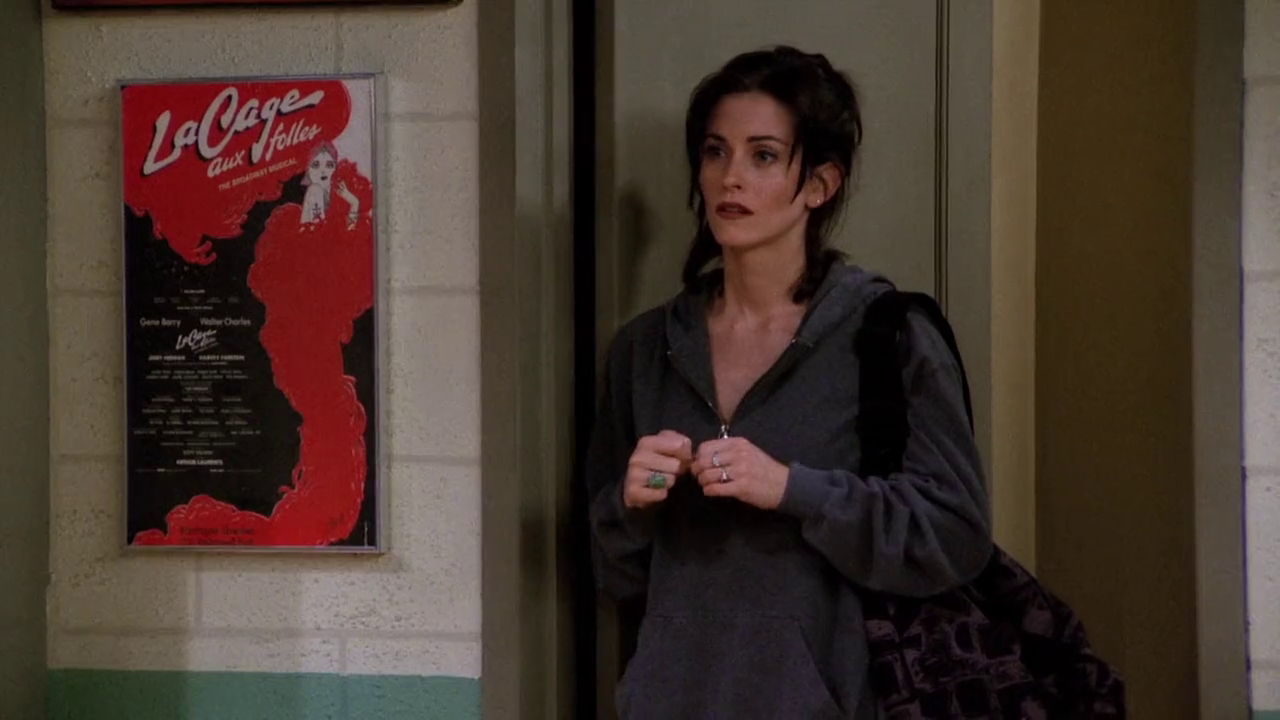
\includegraphics[trim={0 6cm 0 1cm,}, clip, width=\paperwidth]{./S01/img/21/la-cage-aux-folles.png}
    % \caption{La Cage Aux Folles\label{fig:la-cage-aux-folles}}
  \end{adjustwidth}
\end{figure}

\saveparinfos
\noindent
\begin{minipage}[c]{0.5\textwidth}\useparinfo

Monica volta a visitar a classe de dança e na entrada é possível ver o
poster de \emph{La Cage Aux Folles} (1983), musical da \emph{Broadway}
baseado numa peça teatral francesa de mesmo nome. Em 1978 é lançado um
filme e fica conhecido no Brasil como \emph{A Gaiola das Loucas}, e
conta a história de um pai que se descobre gay e é gerente de uma casa
noturna, e que irá conhecer os pais ultra conservadores da noiva de seu
filho.\footnote{\sloppy La Cage Aux Folles - IBDB - Internet Broadway Database (Inglês). \url{https://www.ibdb.com/broadway-show/la-cage-aux-folles-5126}}

\end{minipage}\hfill
\begin{minipage}[c]{0.45\textwidth}

\begin{figure}
  \centering
  \begin{tikzpicture}
    \node [inner sep=0pt] at (0,0) {
      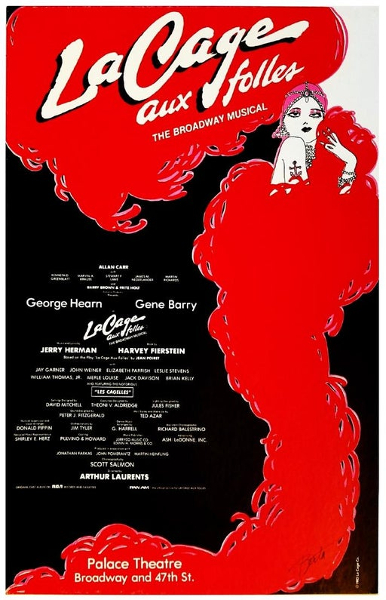
\includegraphics[width=0.7\textwidth,keepaspectratio]{./S01/img/21/la-cage-aux-folles-poster.jpg}
    };
    \draw [white, rounded corners=\ClipSep, line width=\ClipSep]
    (current bounding box.north west) --
    (current bounding box.north east) --
    (current bounding box.south east) --
    (current bounding box.south west) -- cycle
    ;
    \end{tikzpicture}
    \caption{La Cage Aux Folles - Poster\label{fig:la-cage-aux-folles-poster}}
\end{figure}

\end{minipage}

A história é semelhante a vivida por Chandler, onde seu pai, Charles, se
descobre gay após ter tido um filho.

\hypertarget{mercutio}{%
\section{Mercutio}\label{mercutio}}

\begin{figure}[!ht]
  \begin{adjustwidth}{-\oddsidemargin-1in}{-\rightmargin}
    \centering
    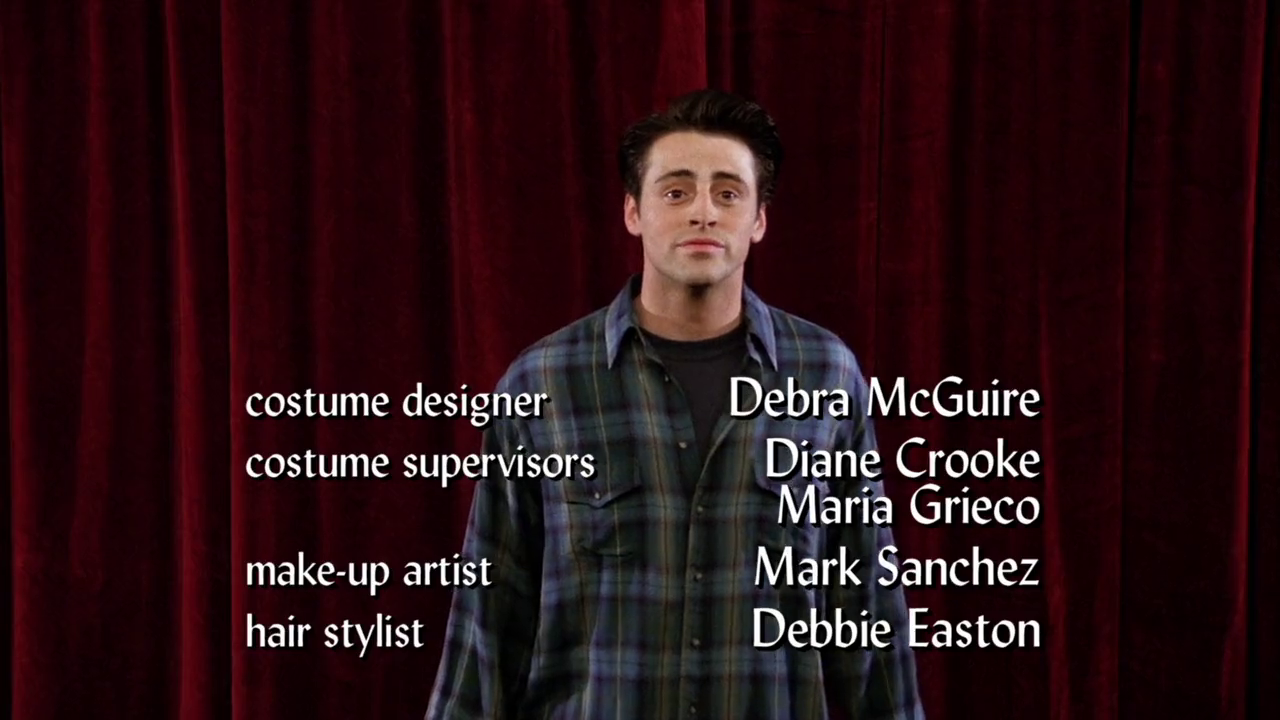
\includegraphics[trim={0 6cm 0 2cm,}, clip, width=\paperwidth]{./S01/img/21/mercutio.png}
    % \caption{Mercutio\label{fig:mercutio}}
  \end{adjustwidth}
\end{figure}

Joey vai a uma audição para tentar o papel de \emph{Mercutio},
personagem, originalmente, do livro \emph{Romeo and Juliet} (1597) de
\emph{William Shakespeare} (1564-1616), o melhor amigo de \emph{Romeo}
na história.\footnote{\sloppy Mercutio - Wikipédia (Inglês). \url{https://en.wikipedia.org/wiki/Mercutio}}
